\documentclass{rpd}
\usepackage{pgf}
\usepackage{tikz}

\madeby{Павловым Александром Викторовичем, доцентом каф. ИТ, к.~ф.-м.~н.}
\kafedra{информационных технологий}
\disciplinecode{Б2.Б.7}
\discipline{Теория автоматов и формальных языков}
\program{010300.62 --- Фундам. информатика и информ. технологии} 
\degree{бакалавр} 
\profile{Сетевые технологии} 
\rpdyear{2013}

\begin{document}

\maketitle

\section{Требования к результатам освоения дисциплины (модуля)}

    Преподавание дисциплины «\@discipline» имеет следующие \emph{цели}:
    \begin{enumerate}
        \item дать введение в идеи и методы теории формальных языков;
        \item ознакомить с основными способами задания и анализа регулярных языков;
        \item ознакомить с основными способами задания и анализа контекстно-свободных языков.
    \end{enumerate}

    \bigskip Дисциплина участвует в формировании следующих \emph{компетенций} выпускника:
    \begin{itemize}
        \item
        ОК-7 --- владеть культурой мышления, аргументировано и ясно строить устную и письменную речь;
        \item
        ОК-10 --- способность использовать основные законы естественнонаучных дисциплин в профессиональной деятельности, применять методы математического анализа и моделирования, теоретического и экспериментального исследования;
        \item
        ПК-2 --- способность профессионально решать задачи производственной и технологической деятельности с учетом современных достижений науки и техники, включая: разработку алгоритмических и программных решений в области системного и прикладного программирования; разработку математических, информационных и имитационных моделей по тематике выполняемых исследований; создание информационных ресурсов глобальных сетей, образовательного контента, прикладных баз данных; разработку тестов и средств тестирования систем и средств на соответствие стандартам и исходным требованиям; разработку  эргономичных человеко-машинных интерфейсов (в соответствии с профилями)
        \item
        ПК-4 --- способность понимать и применять в исследовательской и прикладной деятельности современный математический аппарат, фундаментальные концепции и системные методологии, международные и профессиональные стандарты в области информационных технологий, способность использовать современные инструментальные и вычислительные средства (в соответствии с профилем подготовки)
        \item
        ПК-8 --- способность профессионально владеть базовыми математическими знаниями и информационными технологиями, эффективно применять их для решения научно-технических задач и прикладных задач, связанных с развитием и использованием информационных технологий.
        \item
        ПК-17 --- детальное знание методов и базовых алгоритмов обработки информационных структур, методов анализа сложности алгоритмов
        \item
        ПК-19 --- понимание концепций, синтаксической и семантической организации, методов использования современных языков программирования
    \end{itemize}
    
    \bigskip
    После успешного освоения дисциплины студент должен:\\
    \emph{Знать:}
    \begin{itemize}
        \item 
        определение, основные способы задания и свойства автоматных языков;
        \item 
        определение, основные способы задания и свойства контестно-свободных языков;
        \item
        алгоритмы, используемые для определения принадлежности заданной строки заданному регулярному или КС-языку.
    \end{itemize}
    \emph{Уметь:}
    \begin{itemize}
        \item 
        строить регулярные выражения для автоматных языков;
        \item 
        понимать и проверять индуктивные доказательства свойств языков, автоматов и грамматик;
        \item
        преобразовывать задание регулярного языка в виде автомата, грамматики, регулярного выражения;
        \item
        приводить КС-грамматику к нормальной форме Хомского;
        \item
        пользоваться в компьютерных программах простыми регулярными выражениями для поиска текста.
    \end{itemize}
    \emph{Владеть навыками:} 
    \begin{itemize}
        \item 
        проверки вхождения заданной строки в язык, заданный конечным автоматом или регулярным выражением; 
        \item 
        чтения грамматик, заданных в форме Бэкуса-Наура и построения примеров строк, выводимых в данной грамматике.
    \end{itemize}   


\section{Место дисциплины (модуля) в структуре ООП ВПО}

    Дисциплина «\@discipline» относится к циклу «Б2. Математический и естественнонаучный цикл», блоку «Б2.Б — Базовая часть».  Данная дисциплина имеет содержательно-методические взаимосвязи со следующими дисциплинами:
    \begin{itemize}
    \item Б3.Б.13 --- математическая логика и теория алгоритмов;
    \item Б2.Б.6 --- математическая логика и теория алгоритмов;
    \item Б3.Б.1 --- алгоритмы и анализ сложности;
    \item Б3.Б.2 --- основы программирования;
    \item Б3.Б.3 --- языки программирования.
    \end{itemize}

    \begin{linktable}
        \@disciplinecode & \@discipline & 
        Регулярные языки. Иерархия Хомского. Контекстно-свободные языки. Языки, распознаваемые машиной Тьюринга. Неразрешимые языки. &  
        --- &
        Б3.В.ОД.1, Б2.Б.6, Б2.Б.7, Б2.Б.8, Б3.Б.1 &
        ОК-10, ПК-2, ПК-4, ПК-8, ПК-15
    \end{linktable}

    \begin{hourtable}
        1 & 1,5 & 54 & 28 & 14 & 14 & -- & 2 & 24 & \raggedleft зачет & 2\\
        \hline
        2 & 3,5 & 99 & 44 & 22 & 22 & -- & 5 & 50 & \raggedleft экзамен & --
    \end{hourtable}

    В первом семестре интерактивное занятие (2ч.) --- построение комбинаторных схем цифровой логики из вентилей в симуляторе-конструкторе для ПК.  


\section{Структура и содержание дисциплины}
    \begin{contentstable}
    \multicolumn{10}{|c|}{I  СЕМЕСТР}\\
    \hline
    1 & 1-2 &   Понятие математического доказательства. Метод матем. индукции &  2 & – & 2 &  – &    & & 2-я нед. – опрос\\ \hline
    2 & 3–6 &   Элементы комбинаторики                                        &  4 & – & 4 & 10 &  1 & & 6-я нед. – КР   \\ \hline
    3 & 7–14 &  Булевы функции I                                              &  8 & – & 8 & 14 &  1 & & 14-я нед. – КР \\ \hline
    \multicolumn{10}{|c|}{II  СЕМЕСТР}\\
    \hline
    4 & 1–4 &   Булевы функции II                                             &  6 & – & 6 &  4 &  1 & & 4-я нед. – КР   \\ \hline
    5 & 4–13 &  Элементы теории графов                                        &  8 & – & 8 & 24 &  2 & & 8-я нед. – КР   \\ \hline
    6 & 14–19 & Знакомство с~формальными языками                              &  4 & – & 4 & 16 &  1 & & 14-я нед. – КР \\ \hline
    7 & 20–23 & Элементы теории алгоритмов                                    &  4 & – & 4 &  6 &  1 & & 18-я нед. – КР \\ \hline
    \multicolumn{3}{|r|}{ИТОГО:~}                                             
    & 36 & – &36 & 74 &  7 & &
    \end{contentstable}

    \begin{srstable}
    2 & Комбинаторные объекты и~дискретная вероятность                & ИЗ & 10 & GD & ЛП \\ \hline
    3 & Булевы функции I                                              & ИЗ & 14 & GD & ЛП \\ \hline
    4 & Булевы функции II                                             & ИЗ &  4 & GD & ЛП \\ \hline
    5 & Элементы теории графов                                        & ИЗ & 24 & GD & ЛП \\ \hline
    6 & Знакомство с~формальными языками                              & ИЗ & 16 & GD & ЛП \\ \hline
    7 & Элементы теории алгоритмов                                    & ИЗ &  6 & GD & ЛП
    \end{srstable}
    {\small ИЗ --- решение задач по индивидуальным вариантам, GD --- система Google Drive, ЛП --- личный прием заданий.}
    
    \subsection*{Тематика письменных работ}
        \begin{enumerate}
        \item
        Опрос по теме <<Понятие математического доказательства. Метод математической индукции>>: найти ошибки в доказательстве, объяснить обоснования последовательных шагов в примере доказательства по индукции.  
        \item
        Контрольная работа по теме <<Комбинаторика>>: размещения, сочетания, перестановки, разбиения, правила суммы и произведения, правило включений и исключений.
        \item
        Контрольная работа по теме <<Булевы функции I>>: количество различных булевых функций, удовлетворяющих определенным условиям; преобразования к нормальной форме; фиктивные и существенные переменные; построение СДНФ и СКНФ и по таблицам; разложение Шеннона.
        \item
        Контрольная работа по теме <<Булевы функции II>>: полиномы Жегалкина, замкнутые классы функций, теорема Поста о полных системах функций.
        \item
        Контрольная работа по теме <<Элементы теории графов>>: связность, лемма о рукопожатиях, свойства деревьев, обходы, планарные графы, паросочетания.
        \item
        Контрольная работа по теме <<Знакомство с~формальными языками>>: распознавание принадлежности слова языку, построение конечных автоматов, построение регулярных выражений, теорема о детерминизации.
        \item
        Контрольная работа по теме <<Элементы теории алгоритмов>>: построение простых машин Тьюринга, исполнение простых программ для МТ.
    \end{enumerate}
    

\section{Организация текущего контроля успеваемости и промежуточной аттестации по дисциплине (модулю)}

    \subsection{Описание и примеры оценочных средств}


    \subsubsection*{Опрос по теме <<Понятие математического доказательства. Метод математической индукции>>}

        \begin{enumerate}
        \item
        Найдите ошибки в следующем доказательстве. 1/8 > 1/4, так как:
        \begin{align*}
            3 &> 2\\
            3 \log_{10}\frac{1}{2} &> 2 \log_{10}\frac{1}{2} \\
            \log_{10}\left(\frac{1}{2}\right)^3 &> \log_{10}\left(\frac{1}{2}\right)^2\\
            \left(\frac{1}{2}\right)^3 &> \left(\frac{1}{2}\right)^2.
        \end{align*}
        \item
        Заполните пробелы в~обоснованиях шагов доказательства по индукции.
        \[ 1^2 + 2^2 + \ldots + n^2 = \frac{n(n+1)(2n+1)}{6}.\]

        Обозначим утверждение о равенстве для данного $n$ через $P(n)$.

        \emph{База индукции}. $P(1) = 1$, так как \rule{3cm}{.6pt}.

        \emph{Шаг индукции}. Предположим, для некоторого $k \geqslant 1$ имеют место $P(1)$,  \ldots $P(k)$. Докажем, что в этом случае верно и $P(k+1)$. Имеем
        \[ 1^2 + 2^2 + \ldots + (k+1)^2 = \frac{k(k+1)(2k+1)}{6} + (k+1)^2,\]
        так как \rule{3cm}{.6pt}.

        \[ 1^2 + 2^2 + \ldots + (k+1)^2 = \frac{2k^3 + 3k^2 + k}{6} + \frac{6k^2 + 12k + 6}{6} = \frac{2k^3 + 9k^2 + 13k + 6}{6},\]
        так как \rule{3cm}{.6pt}. С другой стороны,
        \[
        (k+1)(k+2)(2(k+1)+1) = 2k^3 + 9k^2 + 13k + 6.
        \]
        \end{enumerate}
        
        
    \subsubsection*{Контрольная работа по теме <<Комбинаторика>>}

        \begin{enumerate}
        \item
        Сколькими способами можно составить шестизначное число, в котором на четных местах (2-м, 4-м, 6-м) стоят нечетные цифры, а на нечетных местах — четные. Например, 278125~--- одно из таких чисел .
        \item
        а) У ребенка 8 листов с разными рисунками. Есть папка для рисунков с пронумерованными прозрачными кармашками, но кармашков только 5. Сколькими способами он может положить по одному рисунку в каждый кармашек?\\
        б) В президиуме на сцене стоят в ряд 14 кресел, в президиум садятся 6 человек. Сколькими способами они могут сесть на кресла?
        \item
        Сколькими способами можно выбрать 6 человек из 12, если среди них 4 девушки и хотя бы одна должна быть выбрана?
        \item
        Сколькими способами можно переставить буквы слова <<компьютеризация>> так, чтобы никакие две гласные не стояли рядом?
        \item
        Сколько четырехзначных чисел можно составить из цифр числа <<132 131>> (необходимо использовать все шесть цифр)?
        \end{enumerate}
                
    \subsubsection*{Контрольная работа по теме <<Булевы функции I>>}
        \begin{enumerate}
        \item
        Сколько существует булевых функций $f(x_1,x_2,x_3)$ трех
        переменных, которые принимают значение $f=1$, как только $x_3=1$, и почему?
        \item
        Найдите множество единичных значений для функции
        \[
        h(x_1,x_2,x_3,x_4,x_5)= \overline{\bigl(x_3\vee (\bar{x}_5 \sim x_4)\bigr)} \downarrow \bigl((x_2\oplus x_4)x_1\bigr)
        \]
        \item
        Найдите формулу, задающую ту же булеву функцию, но 
        построенную только при помощи $\neg$, $\wedge$, $\vee$
        и не содержащую общих знаков отрицания:
        \[(x \wedge (y \to z)) \downarrow \overline{x \vee y}\]
        \item
        Определите существенные и фиктивные переменные булевой функции
        \[g(x_1,x_2,x_3)=x_1(x_2 \to x_3\bar{x}_1) \vee \bar{x}_1\bar{x}_2 \vee  x_3\bar{x}_1\]
        \item
        Найдите какую-нибудь формулу для функции $f(x_1,x_2,x_3,x_4)$, если известно, что 
        \[f(0,0,0,1) =  f(1,0,1,0) = f(1,1,1,0) = 1,\] 
        а для остальных наборов переменных $f = 0$.
        \end{enumerate}

    \subsubsection*{Контрольная работа по теме <<Булевы функции II>>}

        \begin{enumerate}
        \item
        Представить функцию, заданную вектором $(10111101)$, в виде полинома Жегалкина.
        \item
        Определить, является ли функция с~вектором значений~$(0101010110101010)$ линейной. Если да, то найти ее полином Жегалкина.
        \item
        Дана функция 
        \[
        F(x_1,x_2,x_3) = (\overline{x_1x_2}|x_3\oplus x_1)\vee \overline{x_2x_3x_1}.
        \]
        Если функция не самодвойственная, получить константу путем подстановки на места ее переменных $x$ и $\overline{x}$. Если функция не монотонна, получить функцию $\overline{x}$ путем подстановки на места ее переменных $0$, $1$ и $x$:
        \item 
        Является ли система функций $\{f,g,h\}$ полной? Обоснуйте свой ответ.
        \[
            \alpha_f=(01010111), \alpha_g = (00111001), h(x_1,x_2,x_3) = (\overline{x_1}\sim x_2)\vee x_3
        \]
        \end{enumerate}
        
    \subsubsection*{Контрольная работа по теме <<Графы>>}
        \begin{enumerate}
        \item
        Найдите периферию графа, заданного матрицей смежности\\
        \small
        \[
        \left(
        \begin{array}{ccccccc}
        0&1&0&0&0&0&1\\
        1&0&1&0&0&0&0\\
        0&1&0&1&1&1&0\\
        0&0&1&0&0&0&1\\
        0&0&1&0&0&0&1\\
        0&0&1&0&0&0&1\\
        1&0&0&1&1&1&0
        \end{array}
        \right).
        \]
        \normalsize
        \item
        Нарисуйте какой-нибудь граф, вершины которого имеют указанные степени, или докажите, что это невозможно:\\
        а)  $(2,2,2,3,3,3,4,4)$,\\
        б)  $(2,2,2,2,3,3,4)$.
        \item
        Нарисуйте граф с матрицей смежности 
        \[
        \left(
        \begin{array}{cccccc}
        0 & 1 & 1 & 0 & 1 & 1\\
        0 & 0 & 1 & 1 & 1 & 1\\
        1 & 1 & 0 & 1 & 1 & 0\\
        0 & 1 & 1 & 0 & 1 & 1\\
        1 & 1 & 1 & 1 & 0 & 1\\
        1 & 1 & 0 & 1 & 1 & 0\\
        \end{array}
        \right)
        \]
        как плоский граф или докажите, что это невозможно.
        \item
        Введите на рисунке вершины так, чтобы он превратился в обыкновенный граф (без кратных ребер). Найдите и выпишите эйлеров цикл (его вершины) в этом графе или докажите, что такого цикла не существует. 
        \newline
        \hbox to \hsize{\hfil{
        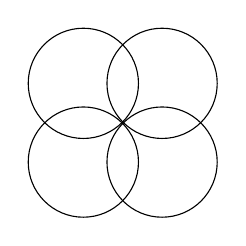
\begin{tikzpicture}
        \draw (0,0) circle (7mm);
        \draw (1cm,0) circle (7mm);
        \draw (0,1cm) circle (7mm);
        \draw (1cm,1cm) circle (7mm);
        \end{tikzpicture}
        }\hfil}

        \item
        Нарисуйте все неизоморфные деревья на 7 вершинах, имеющие хотя бы одну вершину степени 3.
        \item
        В неком родословное древе отображен родоначальник и его прямые потомки (их супруги не отображены). В древе 54 человека. У каждого человека в дереве не более 3 детей. Какова минимально и максимально возможная высота дерева?
        \end{enumerate}
        


    \subsubsection{Для промежуточной аттестации}
        \subsubsection*{Примерный список экзаменационных вопросов}
        \newlist{examquestions}{enumerate}{1}
        \setlist[examquestions]{resume,nolistsep,labelindent=0pt,leftmargin=\parindent,label=\arabic*.}
        \textbf{Комбинаторика}
            \begin{examquestions}
            \item
            Правило сложения и правило умножения.
            \item
            Число размещений с повторениями.
            \item
            Число перестановок из $n$ символов.
            \item
            Число сочетаний из $n$ по $k$.
            \item
            Формула включений и исключений.
            \end{examquestions}

            \smallskip
            \textbf{Булевы функции}
            \begin{examquestions}
            \item
            Булева функция. Таблица истинности. Функции $\vee, \wedge, \to, \neg, \vert, \downarrow$. 
            \item
            Число всевозможных булевых функций от n переменных.
            \item
            Фиктивные и существенные переменные.
            \item
            Основные эквивалентности. Формула с тесными отрицаниями. 
            \item
            ДНФ и КНФ, СДНФ и СКНФ, их построение. 
            \item
            Полиномы Жегалкина. Существование полинома Жегалкина для произвольной булевой функции.
            \item
            Замкнутые и полные классы функций. Некоторые замкнутые классы.
            \item
            Теорема Поста.
            \end{examquestions}

            \smallskip
            \textbf{Теория графов}
            \begin{examquestions}
            \item
            Графы, орграфы, мультиграфы. Инцидентность.Степень вершины. Представление графа матрицей смежности. Представление графа списками смежных вершин.
            \item
            Сумма степеней вершин графа
            \item
            Маршрут, цепь, простая цепь, цикл. Расстояние между вершинами в графе. Обхват и диаметр графа.
            \item
            Связность. Связная компонента графа. Нахождение всех вершин связной компоненты данной вершины. Алгоритмы обхода графа в ширину и в высоту. Сильная связность. Нахождение компонент сильной связности.
            \item
            Реберная и вершинная связность.
            \item
            Помеченные графы. Алгоритм Дейкстры.
            \item
            Деревья. Теорема о критериях дерева (связности и $V=E+1$, ацикличность и $V=E+1$, связность и единственность простого пути). Алгоритмы Прима и Крускала.
            \item
            Эйлеровы графы. Критерии эйлеровости. Построение эйлерового цикла.
            \item
            Гамильтоновы графы. Каждый гамильтонов граф двусвязен. Каждый негамильтонов граф содержит тэта-подграф. Эйлеровость и гамильтоновость.
            \item
            Планарные и плоские графы. Формула Эйлера. Максимальное число ребер в планарном графе. Наличие вершин степени $\le 5$ в планарном графе. Непланарность $K_3$ и $K_{5,5}$. Теорема Понтрягина — Куратовского (без доказательства).
            \item
            Раскраски графа. Теорема о пяти красках. Проблема четырех красок (без доказательства).
            \end{examquestions}

            \smallskip
            \textbf{Формальные языки}
            \begin{examquestions}
            \item
            Конечный автомат, его язык. ДКА и НКА, построение ДКА, эквивалентного данному НКА. Автоматные языки. Замкнутость класса автоматных языков относительно операций пересечения, объединения и разности.
            \item
            Лемма о разрастании для автоматных языков. Примеры неавтоматных языков.
            \item
            Регулярное выражение. Эквивалентность регулярных выражений и конечных автоматов.
            \item
            Регэкспы. Расширенные регэкспы. 
            \item
            Грамматики. Контекстно-свободные, контекстно-зависимые, линейные, праволинейные грамматики. Включения.
            \item
            Форма Бэкуса-Наура записи КС-грамматик.
            \end{examquestions}

            \smallskip
            \textbf{Теория алгоритмов}
            \begin{examquestions}
            \item
            Машина Тьюринга. Вычисление числовых функций на машине Тьюринга. Правильное вычисление. Композиция машин. Основные служебные машины. Тезис Тьюринга.
            \item
            Примеры алгоритмически неразрешимых задач.
            \end{examquestions}

    \subsection{Балльно-рейтинговая система по дисциплине (модулю)}

    \vskip-8mm
    ~
    \begin{table}[H]
    \caption{Лист контрольных мероприятий по дисциплине}
    \begin{tabular}{|>{\raggedright}p{19.5em}|r|r|r|c|r|}
    \hline
    \multicolumn{1}{|c|}{\multirow{2}{*}[-6pt]{Модули}} &
    \multicolumn{3}{p{13ex}|}{\centering Текущий контроль}&
    \multicolumn{1}{c|}{\multirow{2}{*}[-3pt]{\parbox{10ex}{\centering Промежу\-точный контроль}}}&
    \multicolumn{1}{c|}{\multirow{2}{*}[-3pt]{\parbox{11ex}{\centering Итого по дисциплине}}}
    \\
    \cline{2-4}
    & П & ИЗ & КР & & \\
    \hline
    \multicolumn{6}{|c|}{I СЕМЕСТР}
    \\
    \hline
    1. Понятие матем. док-ва. Индукция       &  3 & 10 & -- & \multirow{3}{*}[-.3ex]{зачет} & \multirow{3}{*}[-.5ex]{100}
    \\ \cline{1-4}
    2. Элементы комбинаторики                & ~3 & 20 & 15 & &
    \\ \cline{1-4}
    3. Булевы функции I                      & ~4 & 30 & 15 & &                               
    \\ \hline
    \multicolumn{6}{|c|}{II СЕМЕСТР}
    \\ \hline
    4. Булевы функции II                     &  2 & 12 &  4 & &  \multirow{3}{*}[-1.2ex]{100}
    \\ \cline{1-4}
    5. Элементы теории графов                &  4 & 15 &  4 & экзамен &
    \\ \cline{1-4}              
    6. Знакомство с~формальными языками      &  3 & 12 &  4 & 30 &
    \\ \cline{1-4}              
    7. Элементы теории алгоритмов            &  1 &  6 &  3 & & \\
    \hline
    \end{tabular}
    \medskip\par
    П --- посещение лекций, опросы; ИЗ --- индивидуальные занятия; КР --- контрольные работы
    \end{table}

    Для допуска к зачету в I семестре необходимо набрать не менее 60~баллов из~100.
    Для допуска к экзамену во~II~семестре необходимо набрать не менее 45~баллов, из 70, предусмотренных за~текущую работу.

\newpage
\section[Учебно-методическое и информационное обеспечение]{Учебно-методическое и информационное \\ обеспечение дисциплины (модуля)}
    \begin{littable}
    \multicolumn{5}{|c|}{Основная литература}
        \\ \hline
    1. & Редькин Н.\,П.
        Дискретная математика. 
        СПб.: Лань, 2006. & 
        УМО по класс. унив. обр-ю 010200 
        & 10 
        & \hfill --- 
        \\ \hline
    2. & Яблонский С.\,В. 
        Введение в дискретную математику. 
        М.: Высш. школа, 2003. & 
        --- 
        & 23
        & \hfill --- 
        \\ \hline
    \multicolumn{5}{|c|}{Дополнительная литература}
        \\ \hline
    1. & Мальцев И.\,А.
        Дискретная математика. 
        СПб.: Лань, 2011. 
        & --- 
        & \hfill (*) 
        & \hfill --- 
        \\ \hline
    2. & Шевелев Ю.\,П., Писаренко Л.\,А., Шевелев М.\,Ю.
        Сборник задач по дискретной математике.
        СПб.: Лань, 2013. 
        & --- 
        & \hfill (*) 
        & \hfill --- 
        \\ \hline
    3. & Новиков, Ф.\,А.
        Дискретная математика для программистов. 
        СПб.: Питер, 2004.
        & --- 
        & \hfill --- 
        & \hfill 1 
        \end{littable}

    \par $(*)$~--- Доступны в ЭБС <<Лань>>. \texttt{http://e.lanbook.com/}. Условия доступа: авторизация по IP адресам из сети университета. 

    \refstepcounter{table}
    \begin{internettable}
    1. & Основы дискретной математики 
        & М.\,И.~Дехтярь
        & HTML, тесты
        & \ttfamily http://www.intuit.ru/
        studies/courses/
        1084/192/info
    \\ \hline
    2. & Дискретная математика 
        & О.\,П.~Кузнецов
        & видеолекции FLV, тесты
        & \ttfamily http://www.intuit.ru/
        studies/courses/
        1049/317/info
    \end{internettable}

\newpage
\section[Материально-техническое обеспечение ]{Материально-техническое обеспечение \\ дисциплины (модуля)}
    Перечень минимально необходимого для реализации ООП мате\-ри\-аль\-но-тех\-ни\-чес\-ко\-го обеспечения 
    (выписка из ФГОС ВПО 010300 --- <<Фундаментальная информатика и~информационные технологии>>, п.~7.17): 

    \begin{quotation}
    Основная образовательная программа должна обеспечиваться учебно-методической документацией и материалами по всем учебным курсам, дисциплинам (модулям) основной образовательной программы. Содержание каждой из таких учебных дисциплин (модулей) должно быть представлено в сети Интернет или локальной сети образовательного учреждения. 

    Внеаудиторная работа обучающихся должна сопровождаться методическим обеспечением и обоснованием времени, затрачиваемого на ее выполнение. 

    Каждый обучающийся должен быть обеспечен индивидуальным неограниченным доступом к электронно-библиотечной системе, содержащей издания учебной, учебно-методической и иной литературы по основным изучаемым дисциплинам и сформированной на основании прямых договоров с правообладателями.

    Библиотечный фонд должен быть укомплектован печатными и/или электронными изданиями основной учебной литературы по дисциплинам базовой части всех циклов, изданными за последние 10~лет (для дисциплин базовой части гуманитарного, социального и экономического цикла~--- за последние 5~лет), из расчета не менее 25~экземпляров таких изданий на каждые 100~обучающихся.

    Фонд дополнительной литературы помимо учебной должен включать официальные, справочно-библиографические и специализированные периодические издания в расчете 1--2~экземпляра на каждые 100~обучающихся.

    Электронно-библиотечная система должна обеспечивать возможность индивидуального доступа для каждого обучающегося из любой точки, в которой имеется доступ к сети Интернет.

    Оперативный обмен информацией с отечественными и зарубежными вузами и организациями должен осуществляться с соблюдением требований законодательства Российской Федерации об интеллектуальной собственности и международных договоров Российской Федерации в области интеллектуальной собственности. Для обучающихся должен быть обеспечен доступ к современным профессиональным базам данных, информационным справочным и     поисковым системам.
    \end{quotation}

    \begin{table}[H]
    \caption{Материально-техническое обеспечение дисциплины (помещение и оборудование)}
    \begin{tabular}{|c|>{\raggedright}p{7ex}|>{\raggedright}p{5em}|>{\raggedright}p{8em}|>{\raggedright}p{8ex}|p{14ex}|p{11ex}|}
    \hline
    № & 
    \centering Неделя & 
    \centering Раздел (модуль) & 
    \centering Форма организации учебного процесса & 
    \centering Объем часов  &    
    \centering Наименование специализированных~ауд. &
    \centering Перечень оборудования 
    \tabularnewline \hline
    \multicolumn{7}{|c|}{Первый семестр}
    \\ \hline
    1. & 1--14 & все & лаборат. & 14 & компьют. класс & перс. компьютеры 
    \\ \hline
    \multicolumn{7}{|c|}{Второй семестр}
    \\ \hline
    2. & 1--22 & все & лаборат. & 22 & компьют. класс & перс. компьютеры 
    \\ \hline\end{tabular}\end{table}

\newpage
\thispagestyle{empty}
\tableofcontents
\end{document}
